\documentclass{beamer}

\usepackage[utf8]{inputenc}
\usepackage{lmodern}
\usepackage[utf8]{inputenc}
\usepackage{lmodern}
\usepackage{multicol}
\usepackage{listings}
\usepackage{xcolor}
\usepackage{graphicx}
\definecolor{myblue}{RGB}{48, 63, 159}
\setbeamercolor{palette primary}{bg=myblue, fg=white}
\setbeamercolor{structure}{fg=myblue}
\setbeamercolor{frametitle}{bg=myblue, fg=white}
\setbeamercolor{title}{bg=myblue, fg=white}
\setbeamercolor{footlinecolor}{bg=myblue, fg=white}


\defbeamertemplate*{title page}{mytemplate}{
	\vfill
	\begin{center}
		
		\begin{beamercolorbox}[wd=0.8\paperwidth, center, rounded=true, shadow=true]{title}
			\usebeamerfont{title}\inserttitle\par
		\end{beamercolorbox}
		\vspace{2cm}
		
		\usebeamerfont{author}\insertauthor
		\vspace{1cm}
		\usebeamerfont{date}\insertdate
	\end{center}
	\vfill
}


\defbeamertemplate*{frametitle}{mytemplate}{
	\begin{beamercolorbox}[wd=\paperwidth, ht=2.5ex, dp=1.5ex, left]{frametitle}
		\hspace{1em}\usebeamerfont{frametitle}\insertframetitle
	\end{beamercolorbox}
}


\setbeamertemplate{footline}{
	\begin{beamercolorbox}[wd=\paperwidth, ht=2.25ex, dp=1ex]{footlinecolor}
		\hspace{1em}\usebeamerfont{author in footline}\insertshortauthor
		\hfill
		\usebeamerfont{title in footline}\insertshorttitle
		\hfill
		\usebeamerfont{date in footline}\insertdate \hspace{1em} \insertframenumber/\inserttotalframenumber \hspace{0.5em}
	\end{beamercolorbox}
}


\setbeamerfont{author in footline}{size=\tiny}
\setbeamerfont{title in footline}{size=\tiny}
\setbeamerfont{date in footline}{size=\tiny}

\newcommand{\myvec}[1]{\ensuremath{\begin{pmatrix}#1\end{pmatrix}}}
\providecommand{\brak}[1]{\ensuremath{\left(#1\right)}}







\begin{document}
	\title{5.2.55}
	\author{Shriyansh Chawda-EE25BTECH11052}
	\setbeamertemplate{footline}{}
	\frame{\titlepage}
	\begin{frame}{Question}
		Solve the following system of linear equations.\[
		\frac{2}{x} + \frac{3}{y} = 13 \quad \frac{5}{x} + \frac{4}{y} = -2 \]
	\end{frame}
	
	\begin{frame}{Solution}
		Let
		\begin{align}
			u = \frac{1}{x}, \quad v = \frac{1}{y}.
		\end{align}
		The given system becomes
		\begin{align}
			2u + 3v &= 13 \\
			5u + 4v &= -2
		\end{align}
		In matrix form:
		\begin{align}
			\myvec{2 & 3 \\ 5 & 4} \myvec{u \\ v} = \myvec{13 \\ -2}.
		\end{align}
	\end{frame}
	
	\begin{frame}{Solution}
		We solve using Gauss-Jordan elimination. We start with the augmented matrix $[A|\vec{b}]$ and reduce it to $[I|\vec{x}]$.
		\begin{align}
			\left[\begin{array}{cc|c}
				2 & 3 & 13 \\
				5 & 4 & -2
			\end{array}\right]
			&\xrightarrow{R_1 \rightarrow \frac{1}{2}R_1}
			\left[\begin{array}{cc|c}
				1 & \frac{3}{2} & \frac{13}{2} \\
				5 & 4 & -2
			\end{array}\right] \\
			&\xrightarrow{R_2 \rightarrow R_2 - 5R_1}
			\left[\begin{array}{cc|c}
				1 & \frac{3}{2} & \frac{13}{2} \\
				0 & -\frac{7}{2} & -\frac{69}{2}
			\end{array}\right] 
		\end{align}
	\end{frame}
	
	\begin{frame}{Solution}
		Continuing the row reduction:
		\begin{align}
			&\xrightarrow{R_2 \rightarrow -\frac{2}{7}R_2}
			\left[\begin{array}{cc|c}
				1 & \frac{3}{2} & \frac{13}{2} \\
				0 & 1 & \frac{69}{7}
			\end{array}\right] \\
			&\xrightarrow{R_1 \rightarrow R_1 - \frac{3}{2}R_2}
			\left[\begin{array}{cc|c}
				1 & 0 & -\frac{58}{7} \\
				0 & 1 & \frac{69}{7}
			\end{array}\right]
		\end{align}
		The matrix is now in reduced row echelon form.
	\end{frame}
	
	
	\begin{frame}{Solution}
		From the final matrix, we can directly read the solution:
		\begin{align}
			u &= -\frac{58}{7} \\
			v &= \frac{69}{7}
		\end{align}
		Back substituting to find $x$ and $y$:
		\begin{align}
			\frac{1}{x} = -\frac{58}{7} &\implies x = -\frac{7}{58}, \\
			\frac{1}{y} = \frac{69}{7} &\implies y = \frac{7}{69}.
		\end{align}
		Thus, the solution is
		\begin{align}
			\myvec{x \\ y} = \myvec{-\tfrac{7}{58} \\ \tfrac{7}{69}}.
		\end{align}
	\end{frame}
	\begin{frame}{Plot}
		\begin{figure}[H]
			\centering
			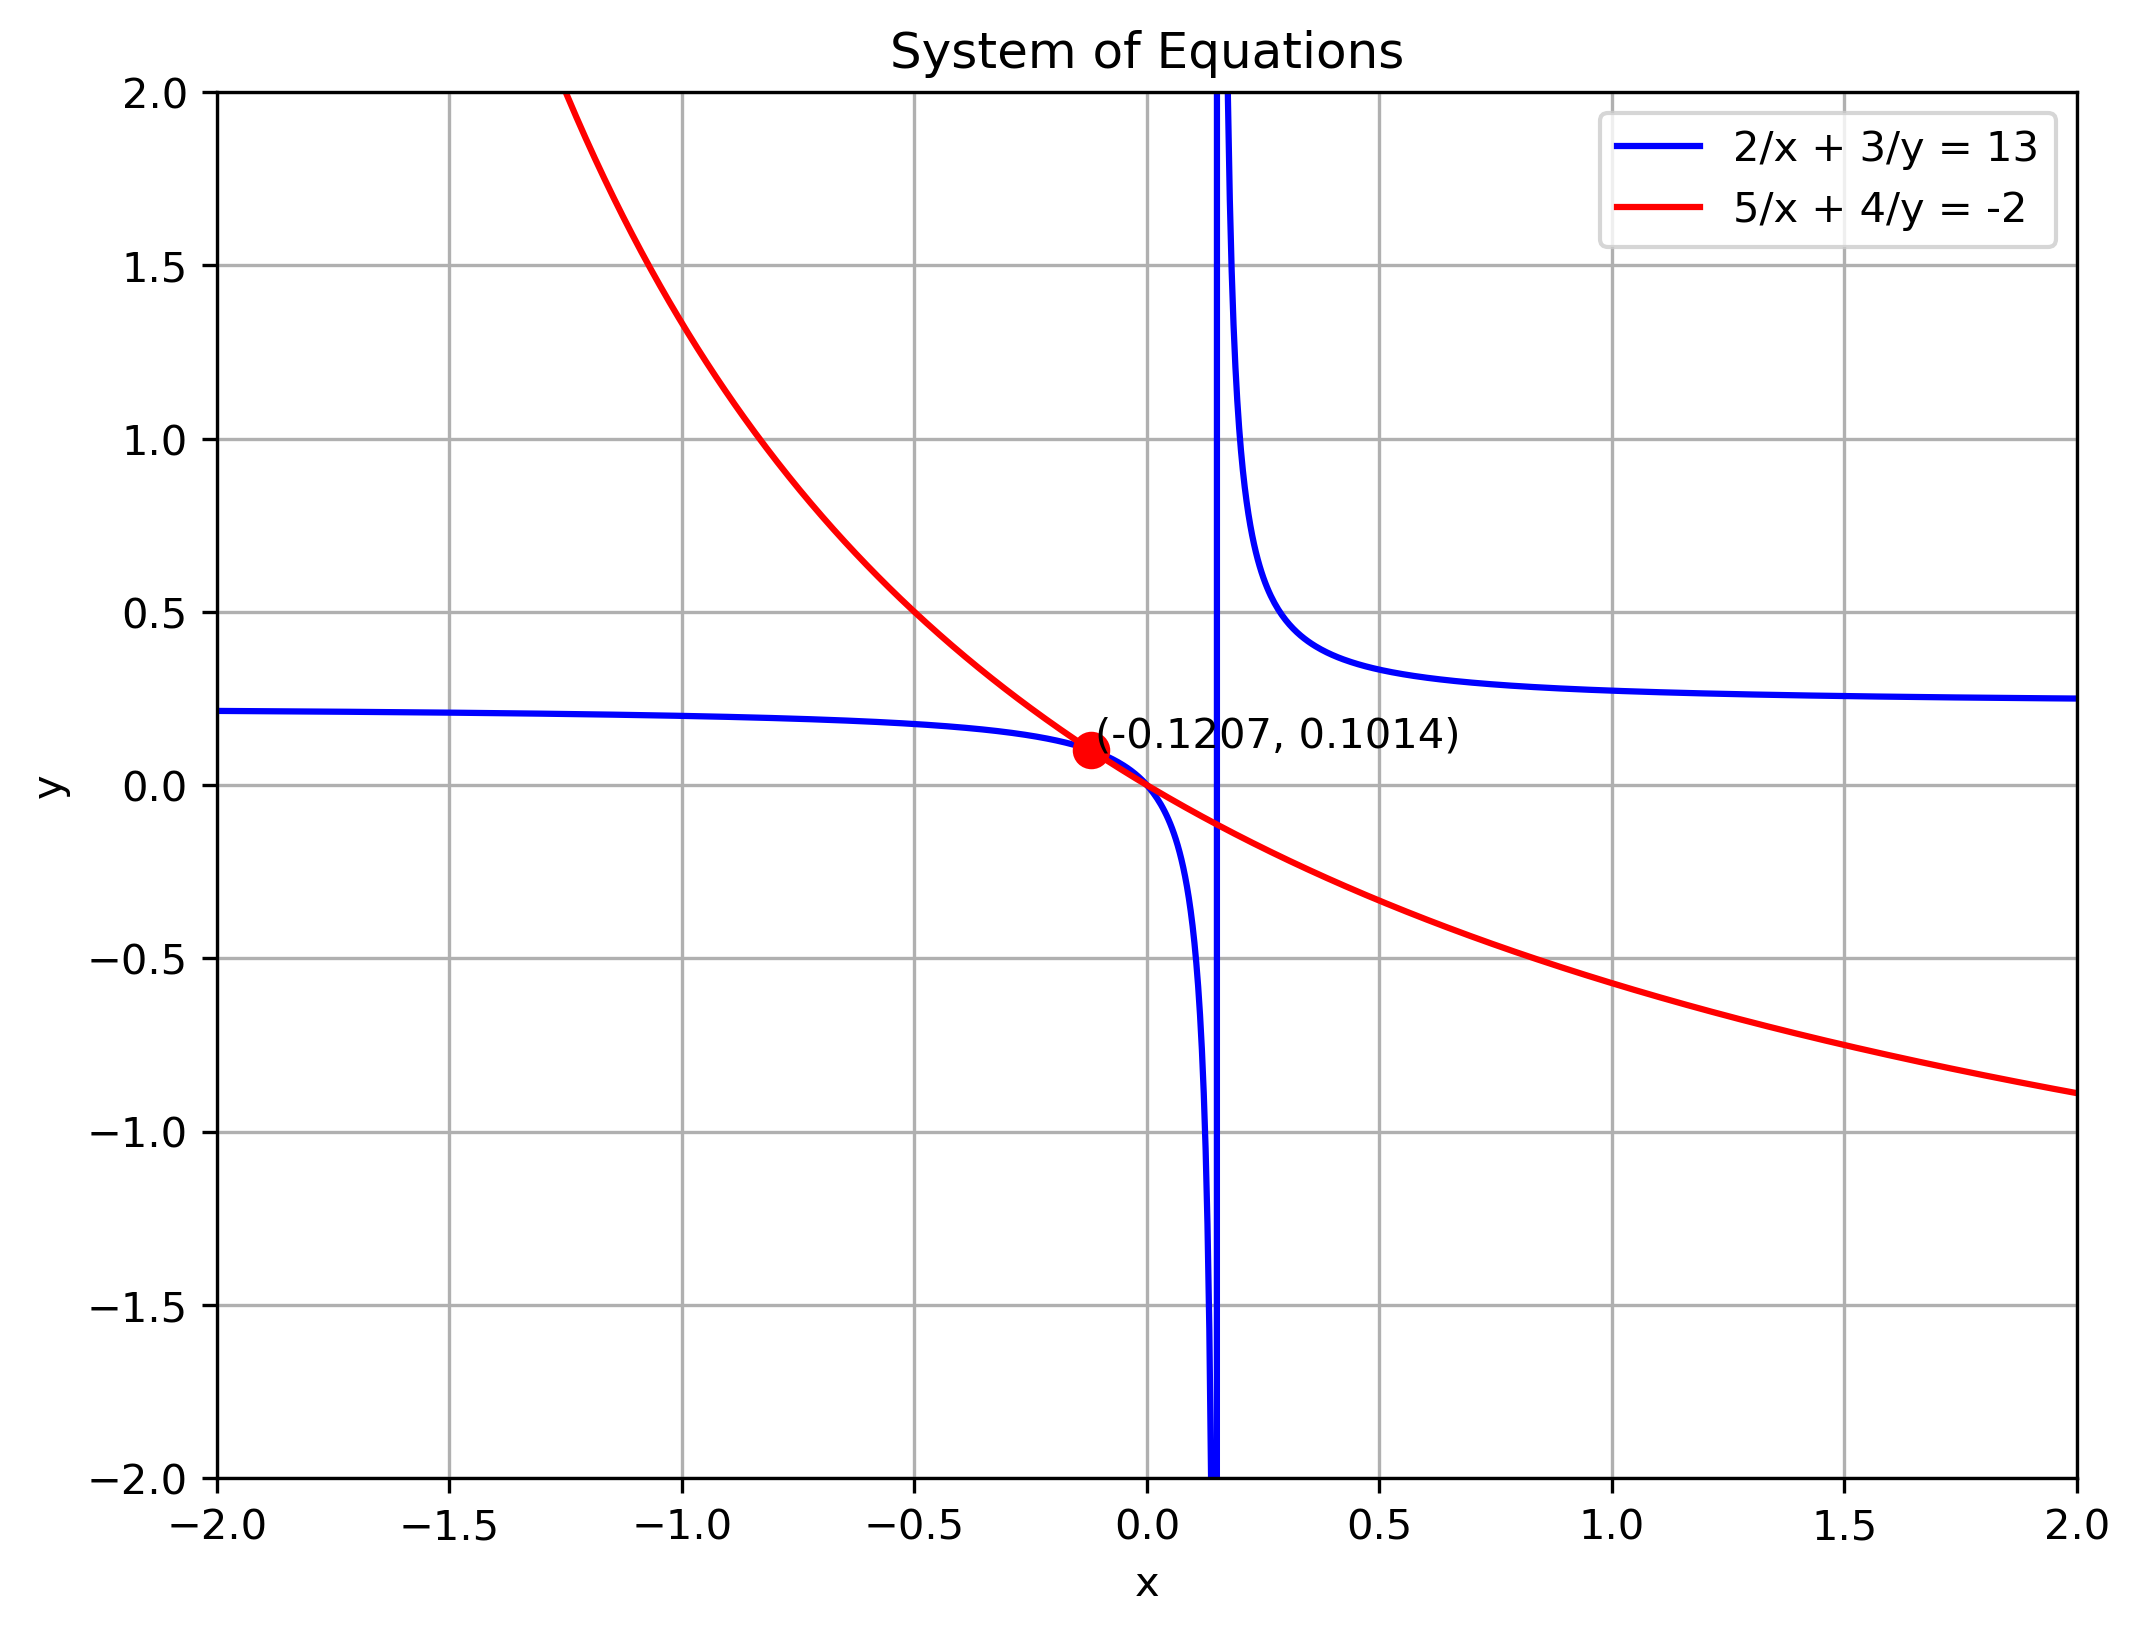
\includegraphics[width=1\linewidth]{../figs/equation_plot}
			\caption{}
			\label{fig:equationplot}
		\end{figure}
		
	\end{frame}
\end{document}